\documentclass[aspectratio=169,12pt]{beamer}

% Theme and color settings
\usetheme{Madrid}
\usecolortheme{default}

% Packages
\usepackage[utf8]{inputenc}
\usepackage{graphicx}
\usepackage{amsmath}
\usepackage{amssymb}
\usepackage{tikz}
\usepackage{hyperref}
\usepackage{listings}
\usepackage{algorithm}
\usepackage{algorithmic}
\usepackage{booktabs}
\usepackage{subfigure}
\usepackage[normalem]{ulem}

\title[AI-Guided DDD at FTAPI]{AI-Assisted Domain Modeling: Enhanced Bounded Context Extraction with LLMs}
\subtitle{A Practical Exploration with FTAPI Software GmbH}
\author[Husein Jusic]{Husein Jusic}
\institute[TUM]{
    \textbf{Supervisor:} Tobias Eisenreich\\
    Chair of Software Engineering\\
    Technical University Munich\\
    \medskip
    \textit{husein.jusic@tum.de}\\
    \textit{h.jusic@ftapi.com}
}
\date{\today}

\begin{document}

% Title Slide
\begin{frame}
    \titlepage
\end{frame}

% Introduction
\begin{frame}{Who am I}
\begin{itemize}
    \item \textbf{Name:} Husein Jusic – Bachelor’s Informatics @ TUM
    \item \textbf{Current Role:} Working student @ FTAPI (\~4 Years)
\end{itemize}
\end{frame}

% Vision vs Reality
\begin{frame}{FTAPI}
    \begin{center}
        
\includegraphics[width=0.2\textwidth]{./img/ftapilogo.png} \\
        \vspace{0.3cm}
        \tiny FTAPI Software GmbH Logo
    \end{center}
\begin{itemize}
    \item FTAPI started in 2010 with the idea: \textit{"One platform to secure all business data exchange."}
    \item Millions of users now rely on FTAPI.
    \item But like many companies, the architecture... did not keep up.
\end{itemize}
\end{frame}

% Problem
\begin{frame}{The Harsh Reality: A Big Ball of Mud}
    \textbf{Antipattern:}
    \begin{center}
        
\includegraphics[width=0.25\textwidth]{./img/BBoM.png} \\
        \vspace{0.3cm}
        \tiny Image generated with \textit{ChatGPT + Sora (OpenAI)}
    \end{center}
\end{frame}
\begin{frame}{The Harsh Reality: A Big Ball of Mud}
\begin{itemize}
    \item \textbf{Platform:} Secutransfer
    \item Monolithic codebase, entangled logic
    \item Hard to scale, harder to understand
    \item Domain knowledge scattered over lots of Services, Managers, ....
\end{itemize}
\end{frame}

% The Plan
\begin{frame}{The Escape Plan: From Monolith to Modulith}
\begin{itemize}
    \item Gradual transformation
    \item Strategy: Domain-Driven Design (DDD)
    \item Goal: Code with clear boundaries and clear responsabilities
\end{itemize}
\end{frame}

% It's Hard
\begin{frame}{Spoiler: This is Really, Really Hard}
\begin{itemize}
    \item Domain knowledge lives in people's heads
    \item Legacy logic spans multiple domains
    \item No consistent language
    \item Time pressure from business side
\end{itemize}
\end{frame}

% Can AI Help?
\begin{frame}{Enter the AI Architect: LLMs in Software Design}
\begin{itemize}
    \item What if AI could help identify bounded contexts?
    \item Extract domain models from large requirement sets?
    \item Help engineers designing software architecutres?
    \item Speed up modularization efforts?
\end{itemize}
\end{frame}

% Research State
\begin{frame}{What the Research Says}
    \begin{itemize}
        \item Fully automated generation of domain models? \\
        \textbf{→ Doesn't work well.}
        
        \item Models are often incomplete
        \item LLMs struggle with identifying relationships between domain concepts
        \item rarely included modeling best practices or complex design patterns
    \end{itemize}
    \vspace{0.5cm}
    \tiny{
        Based on: K. Chen et al., “Automated Domain Modeling with Large Language Models: A Comparative Study,”
        \textit{MODELS 2023}, pp. 162–172. doi: 10.1109/MODELS58315.2023.00037.
    }
\end{frame}

% Semi-automated
\begin{frame}{Not Replacing Engineers – Augmenting Them}
    \textbf{Semi-Automated Domain Modeling with LLM Assistants}:
    \begin{itemize}
        \item Human expert + LLM assistant = \textbf{Better productivity \& quality}
        \item Recent study shows promising results:
        \begin{itemize}
            \item \textcolor{teal}{✓} High precision in suggestions (80\%+ for classes)
            \item \textcolor{teal}{✓} Users report faster modeling compared to manual approach
            \item \textcolor{teal}{✓} Works well even with medium-sized LLMs
            \item \textcolor{orange}{→} Human oversight still essential for accuracy
        \end{itemize}
        \item Key insight: \textbf{Assist, don't replace} – LLMs suggest, humans decide
    \end{itemize}
    \vspace{0.3cm}
    \tiny{
        Based on: D. Prokop et al., "Enhancing Domain Modeling with Pre-trained Large Language Models: An Automated Assistant for Domain Modelers,"
        \textit{ER 2024}, LNCS 15238, pp. 235–253, 2025.
    }
    \end{frame}

% Industry relevance
\begin{frame}{Industry Context}

    \begin{itemize}
        \item Few studies analyze real-world, industrial use cases for AI-based domain model generation.
        
        \item Most research is based on synthetic or simplified examples, which limits practical applicability.
        
        \item \textbf{My Hypothesis:} Integrating Domain-Driven Design (DDD) into AI-assisted model generation could improve architectural quality.
        
        \item \textbf{Why?} DDD provides a structured and context-aware foundation — giving AI a clear "path" for modeling that current approaches lack.
    \end{itemize}
    
\end{frame}

\begin{frame}{In Progress: Preparation}
    \begin{itemize}
        \item \textbf{Prompt Engineering:} Designed and refined a diverse set of prompts to guide the LLM effectively through different DDD stages.
        \item \textbf{Requirements:} Collected and analyzed detailed requirements from the platform.
        \item \textbf{Workflow:} Initiated the implementation of a Spring Boot–based AI application to orchestrate the domain modeling pipeline.
    \end{itemize}
\end{frame}

\begin{frame}{In Progress: Defining a Workflow to Create Architecture Candidates}
    \centering
    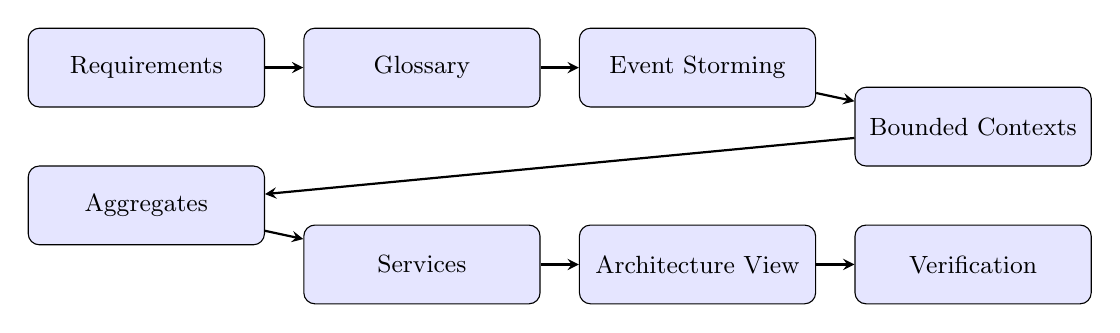
\begin{tikzpicture}[
        every node/.style={align=center, font=\small, minimum height=1cm},
        arrow/.style={->, thick, >=stealth},
        box/.style={rectangle, draw=black, fill=blue!10, rounded corners, minimum width=3cm, minimum height=1cm}
    ]
        % Top row
        \node[box] (req) at (0, 0) {Requirements};
        \node[box] (glossar) at (3.5, 0) {Glossary};
        \node[box] (storming) at (7, 0) {Event Storming};
        \node[box] (bc) at (10.5, -0.75) {Bounded Contexts};

        % Bottom row
        \node[box] (agg) at (0, -1.75) {Aggregates};
        \node[box] (svc) at (3.5, -2.5) {Services};
        \node[box] (arch) at (7, -2.5) {Architecture View};
        \node[box] (verify) at (10.5, -2.5) {Verification};

        % Top row arrows
        \draw[arrow] (req) -- (glossar);
        \draw[arrow] (glossar) -- (storming);
        \draw[arrow] (storming) -- (bc);

        % Connection from top to bottom
        \draw[arrow] (bc) -- (agg);

        % Bottom row arrows
        \draw[arrow] (agg) -- (svc);
        \draw[arrow] (svc) -- (arch);
        \draw[arrow] (arch) -- (verify);
    \end{tikzpicture}

    \vspace{0.5cm}
    \textit{“LLM supports the entire domain modeling pipeline – from raw text to architecture candidates.”}
\end{frame}

\begin{frame}{TBD: Next Steps}
    \begin{itemize}
        \item \textbf{Generate} – Derive bounded context candidates from collected requirements.
        \item \textbf{Evaluate} – Assess both the generation process and the resulting artifacts.
        \item \textbf{Verify} – Validate outcomes through interviews with experienced Domain-Driven Design practitioners.
    \end{itemize}
\end{frame}

% The Goal
\begin{frame}{The Goal}
    \textbf{Can AI help to escape from the monolith faster and better?}
    \textbf{Research Questions:}
    \begin{itemize}
        \item How effectively can Large Language Models (LLMs) identify and define viable bounded contexts that align with complex domain-specific requirements?
        \item To what extent do bounded contexts and domain models identified by LLMs compare in quality and applicability with those created by experienced DDD practitioners when analyzing complex application requirements?
    \end{itemize}
\end{frame}

% End Frame
\begin{frame}{Questions?}
    \centering
    \vspace{2cm}
    \Huge
    \textbf{Any questions or thoughts?}
    
    \vspace{1cm}
    \large
    I’m happy to discuss!
\end{frame}

%
\begin{frame}{Backup: Domain-Driven Design (DDD)}
    \begin{itemize}
        \item \textbf{What is DDD?} \\
        A software design approach focusing on modeling complex domains based on collaboration between technical and domain experts.
        
        \item \textbf{Key Concepts:} \\
        - Ubiquitous Language \\
        - Bounded Contexts \\
        - Entities and Value Objects \\
        - Aggregates and Repositories
        
        \item \textbf{Why DDD?} \\
        Helps create clear, maintainable architectures aligned with real business needs.
        
        \item \textbf{Relation to AI:} \\
        Provides structure and domain knowledge that can guide AI in generating better, context-aware models.
    \end{itemize}
\end{frame}

\begin{frame}[allowframebreaks]{References}
    \footnotesize
    \begin{thebibliography}{10}

    \bibitem{evans2003domain}
    Eric Evans,
    \newblock \textit{Domain-Driven Design: Tackling Complexity in the Heart of Software},
    \newblock Addison-Wesley, 2003.
    \end{thebibliography}
\end{frame}

\end{document}
